\section{Improving Parameter Estimates by Solving Sequences of SIPs}\label{sec:mud-pde-sequence}
As we proceed from two to five dimensions, being wary of the fact that we are fighting against the curse of dimensionality, we want to be more deliberate with our specification of an initial density.

[TK - write a little bit more here, bring in the content about not considering functions that are too rough]

Fig.~\ref{fig:pde-highd-2d-scatter}.

\subsection{Motivations for a New Initial Density}
Recall from \ref{subsec:pde-example} that two maps were used to solve the SIP: $\qoi^{1D}$ and $\qoi^{2D}$, and MUD points were shown for twenty realizations of noise for each in Figure~\ref{fig:pde-convergence}.
In this figure, we use the updated densities from a solution to the SIP from each of $\qoi^{1D}$ and $\qoi^{2D}$ to give an alternative view to that in \ref{fig:pde-convergence} of the feasible region in $\pspace$.
We normalize our evaluations of the ratio of observed to predicted densities and plot the samples that exceed two thresholds, numerical zero (left), and $1/N$ (right) to give some sense of samples that may come from accept/reject algorithms (since our initial was uniform).

Both scatter-plots exhibit the same geometry, appearing to trace a band through the parameter space.
Fundamentally, at first glance at the left figure, it is already apparent that half of $\pspace$ has been ruled out, and that the correlation structure between the two knots has been discovered.
The samples from $\qoi^{2D}$, however, cluster more tightly around the optimal samples (the ``projection'' here refers to the sample which minimizes the 2-norm to the noiseless data).
The incorporation of two directions instead of one whittles away more of the parameter space as being less relatively likely.
If we were to perform accept/reject, the resulting set would be fairly well constrained to the upper-lefthand corner of the two-dimensional parameter space.

\begin{figure}[htbp]
\centering
  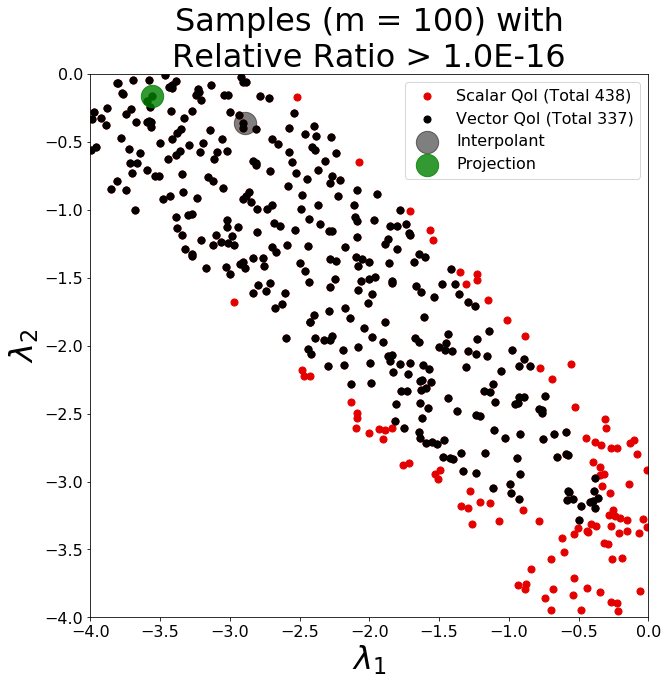
\includegraphics[width=0.45\linewidth]{figures/pde-highd/pde-highd_update_scatter_D2_t1-0E-16.png}
  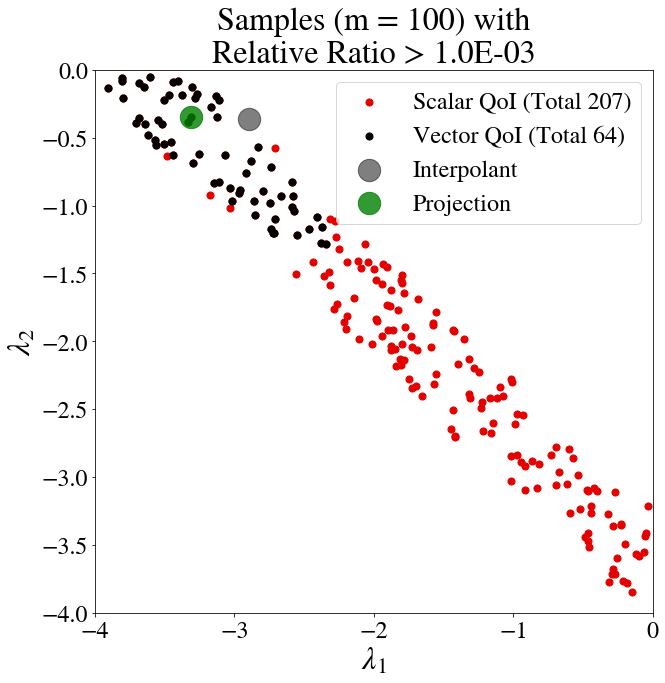
\includegraphics[width=0.45\linewidth]{figures/pde-highd/pde-highd_update_scatter_D2_t1-0E-03.png}
\caption{
100 measurements
}
\label{fig:pde-highd-2d-scatter}
\end{figure}

%%%%%%%%%%%%

Let us take a look at the samples that show up in black on the right of Figure~\ref{fig:pde-highd-2d-scatter} from a different perspective.
These represent samples from the updated density solved by incorporating all 100 measurements.

\begin{figure}[htbp]
\centering
  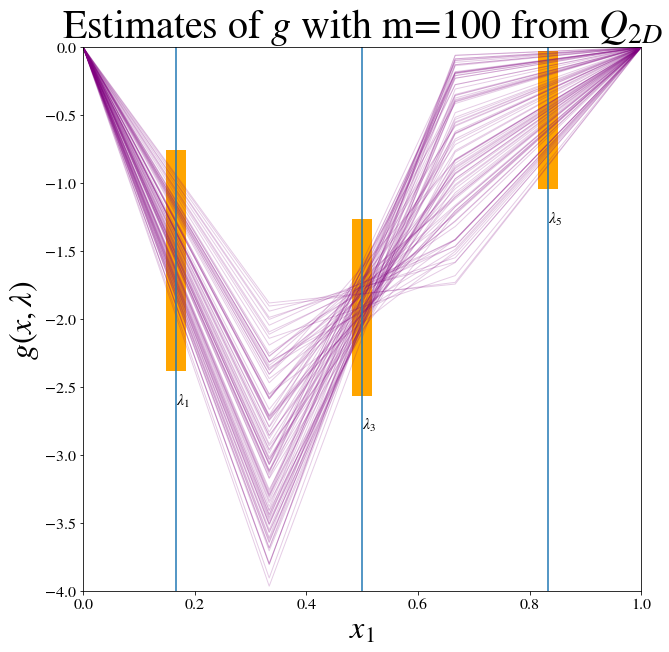
\includegraphics[width=0.675\linewidth]{figures/pde-highd/pde-highd-alt_initial_D5_m100.png}
\caption{
By considering the relationship between the parameters and the types of functions that could be possible given the solution to a 2-D inverse problem, we are able to create a more restricted parameter space in 5-D.
Knowledge of the behavior of $g$ at the boundaries allows for more than half of each of the three remaining intervals to be ruled out as infeasible regions when we look at high-probability samples from the 2-D SIP solution.
}
\label{fig:pde-highd-5d-study}
\end{figure}

In Figure~\ref{fig:pde-highd-5d-study}, we plot the parameter samples whose relative ratios exceeded $1/1000$ sweep out a family of curves that can be used to estimate bounds not only on $\lambda_2$ and $\lambda_4$ (the previous $\lambda_1$ and $\lambda_2$ from the 2-D problem)\---which exhibit correlation structure that we will turn to momentarily\---but also on the remaining three knots.
To form the intervals shown in orange in Fig.~\ref{fig:pde-highd-5d-study}, we take the upper and lower bounds of the curves passing through the vertical lines drawn at the three new knot values.
To be conservative, we multiply our lower bound by $1.2$ and the upper by $0.8$.
With these choices, we are still more than halving the interval-length in each direction as compared to the previous 5-D problem.
One could establish a lower tolerance for accepting likely samples and avoid the multiplication factor, or make any number of other choices for a refined initial density.
However, a thorough exploration of how to best leverage the ratio of observed to predicted densities is left to future work, and will always be highly problem--dependent.


\FloatBarrier
\subsection{Capturing Correlation Structure from 2-D SIP Solution}
For the two remaining directions, we want to capture the correlation structure that we were able to visually identify in Fig.~\ref{fig:pde-highd-2d-scatter} and impose a uniform density over the support of the set.
To achieve this desired refinement of an initial density, we perform a singular-value decomposition on the likely samples from the scalar--valued 2-D solution, since there are so many more samples\footnote{ The scalar-valued contour was found to better characterize the direction of the equivalence class, suggesting perhaps a justifiable use for solving the problem with it. We could have formed an estimate of the updated density from using the vector--valued QoI and sampled from that instead. Many such approaches can be looked into in the future and are briefly discussed in the last section of this chapter.}.
The singular vectors are used to transform the vector-valued samples, and a uniform sampling is performed over the rectangular bounding box for these points, shown in the center of Figure~\ref{fig:pde-highd-2d-study}.
These generated samples, however, leave $\pspace$ when transformed back to their native space, as seen in the left panel.
To ameliorate this problem, we instead perform sampling in a while-loop, sampling from this uniform box and rejecting any that would get mapped back outside $\pspace$, until we reach our desired thousand samples.


\begin{figure}[htbp]
\centering
  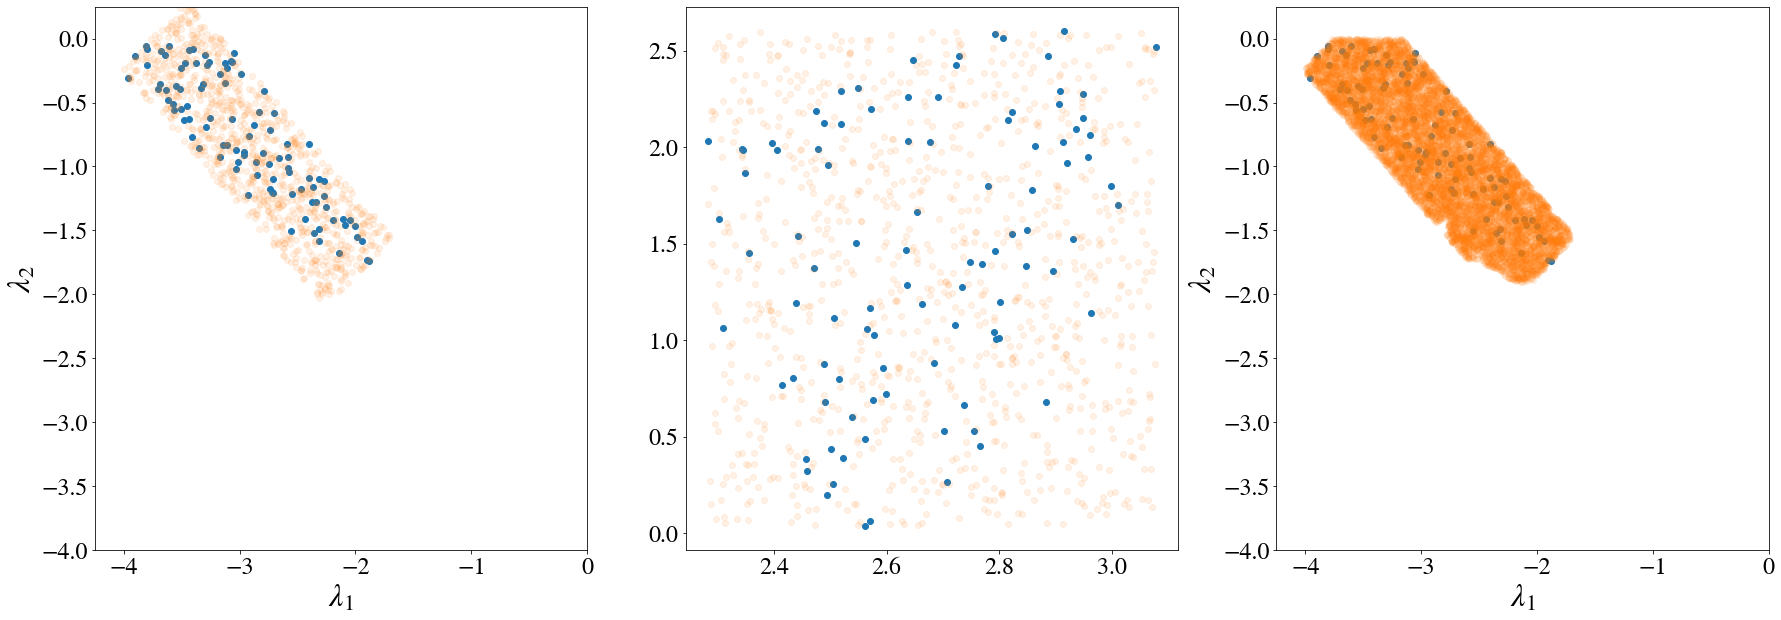
\includegraphics[width=0.95\linewidth]{figures/pde-highd/pde-highd-alt_initial_D2_m100}
\caption{
Generating proposal samples for the two directions informed by solving the 2-D inverse problem, aided by singular-value decompositions and an ad-hoc sampling procedure.
}
\label{fig:pde-highd-2d-study}
\end{figure}

Analogously speaking, we set out to define a computational open cover for the relatively high-probability samples.
In the center panel of Fig~\ref{fig:pde-highd-2d-study}, there are corner-regions of the space we want to avoid wasting samples on as well, so we reject samples that have squared two-norm greater than $0.05$ from their nearest vector--valued sample.
This sampling procedure produces the set shown in orange on the right side of the figure (ten thousand shown to demonstrate coverage).
We keep one thousand of these 2-D samples, and join them with the three independent uniform sample sets of the same size taken from the intervals shown in Fig.~\ref{fig:pde-highd-5d-study} to form our new initial sample set, the functions from which generate the curves shown in Figure~\ref{fig:pde-highd-alt-initial-5d}.

\begin{figure}[htbp]
\centering
  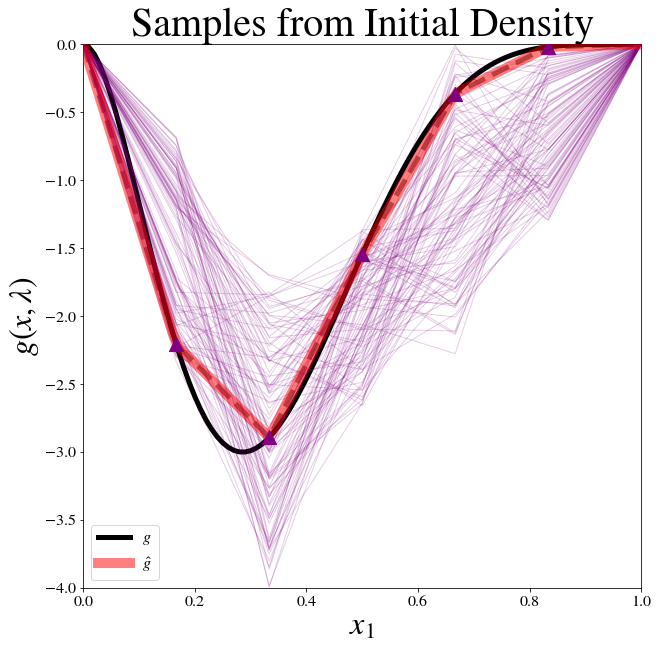
\includegraphics[width=0.675\linewidth]{figures/pde-highd/pde-highd_init_D5-alt}
\caption{
Initial density constructed for the second attempt at the five--dimensional inverse problem, with the structure of solutions learned from the 2-D example incorporated into the selection of bounds in each direction.
}
\label{fig:pde-highd-alt-initial-5d}
\end{figure}

The new initial curves in \ref{fig:pde-highd-alt-initial-5d}\---especially when contrasted to those in Fig.~\ref{fig:pde-highd-initial-5d}\---represent a far more reasonable set of possibilities.
The slope of the functions considered now all only have a single sign change, a marked improvement over the two or three that many samples from \ref{fig:pde-highd-initial-5d} exhibited.
We note that such considerations of smoothness could be avoided by parameterizing $g$ with a basis of some sort, but that problem is beyond the scope of this work.
Another possible improvement would be to incorporate the correlation structure that is present in the three other directions, derivable from a similar SVD-based analysis of the interpolation of the 2-D predictions through the new knot locations.
% However, doing so would require more visual exploration than the authors deem worthwhile to demonstrate the point they are trying to make, which is that better initial densities improve the quality of solutions.

% \begin{figure}[htbp]
% \centering
%   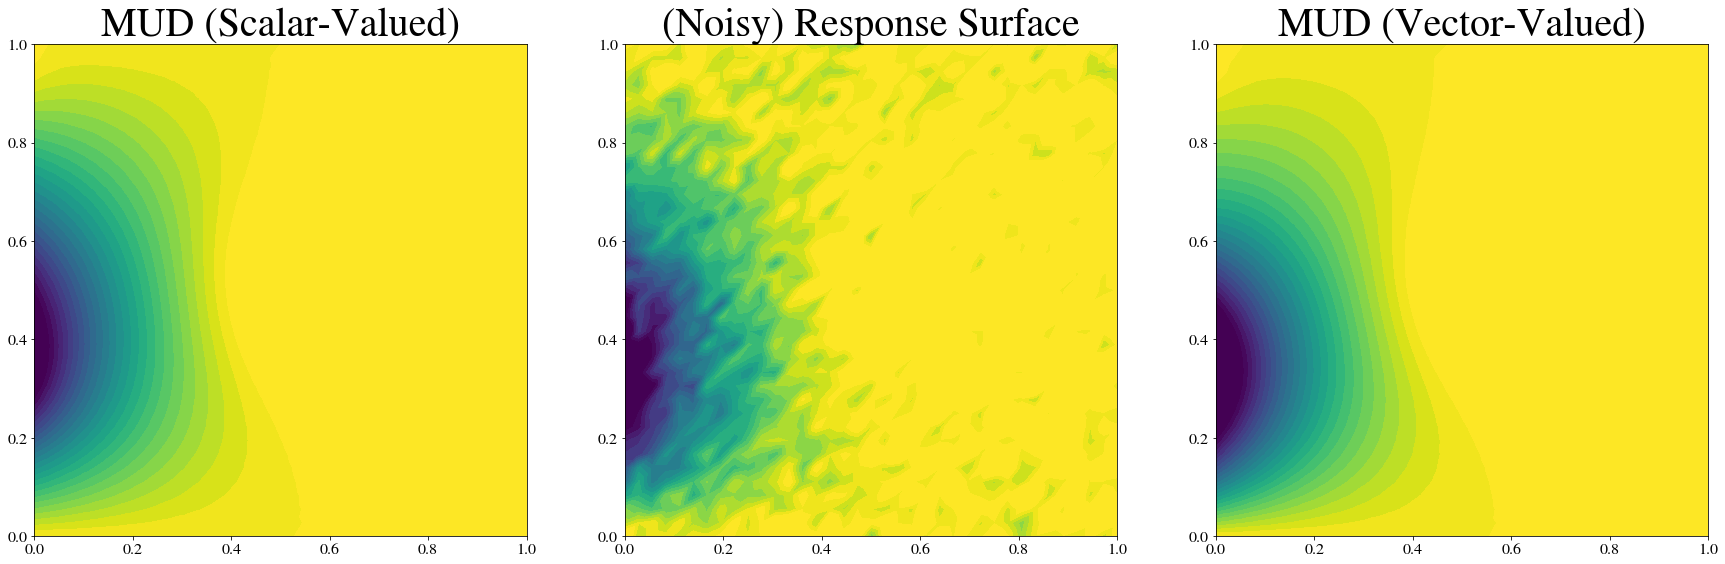
\includegraphics[width=0.95\linewidth]{figures/pde-highd/pde-highd_surf_exmud_D5-alt_m100.png}
%   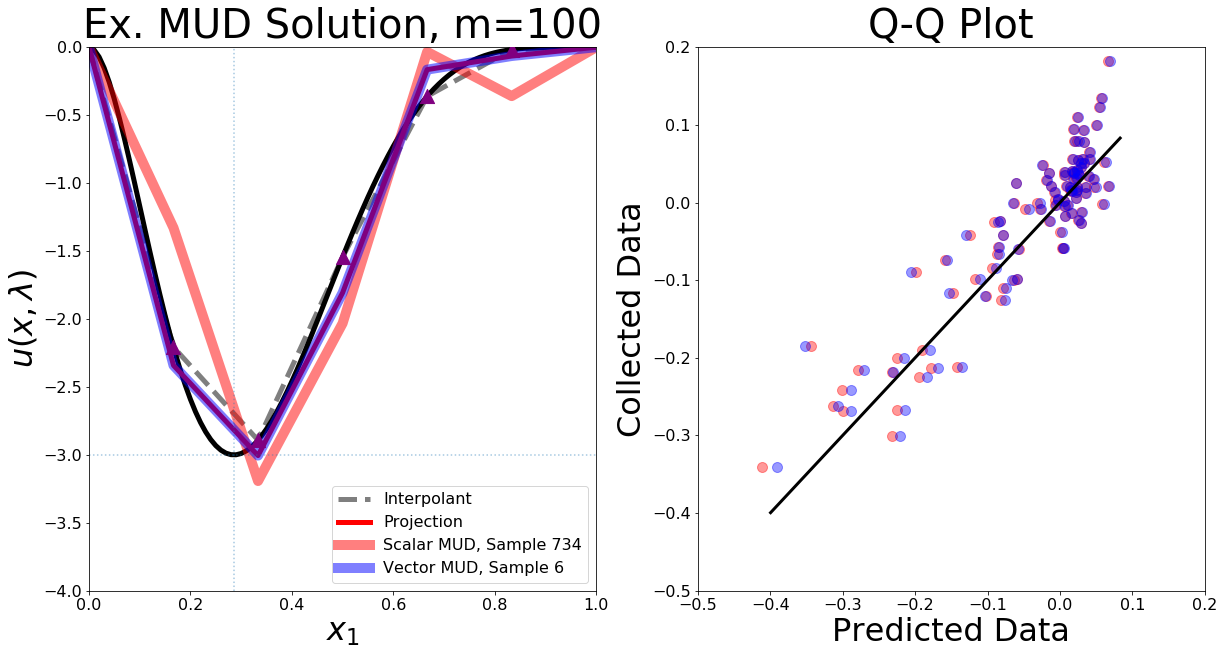
\includegraphics[width=0.9\linewidth]{figures/pde-highd/pde-highd-alt_comp_exmud_D5_m100.png}
% \caption{
% 100 measurements for the revised five--dimensional problem yield substantially better estimates in the eyeball norm.
% }
% \label{fig:pde-highd-5d-alt-example}
% \end{figure}


\subsection{SIP Solutions using New Initial Density}
We now come to the solutions that arise from solving the same five--dimensional inverse problem of interpolating the values of $g$ through equispaced knot points, with both types of maps, in Figure~\ref{fig:pde-highd-5d-alt-mud}.
The difference in comparison to the example solutions in Fig.~\ref{fig:pde-highd-5d-mud} is stark: no longer are the solutions dramatically under-estimating the local minimum of $g$.
To the extent to which they fail to adequately to do is due to the insufficient resolution of five knot points.
Both scalar-- and vector--valued solutions identify the same knot as being the likely minimum, and the latter solution estimates the minima well (horizontal line drawn for reference) in the bottom-right plot.

Once again, we solve our SIP twenty times (for different realizations of noise), to better understand the sensitivity of the parameter estimates produced by the MUD estimator.
We observe some interesting patterns in the curves on the left side of Figure~\ref{fig:pde-highd-5d-alt-mud}.
First, we note that going from scalar-- to vector--valued resolves a significant amount of uncertainty in $\lambda_2$, $\lambda_3$, and $\lambda_4$.
Namely the QoI map appears to stop considering curves which do not have a sufficiently low minimum value.
Second, while the vector--valued MUD solution curves appear to capture the general characteristics of $g$ well, a number of them under-estimated the value at $\lambda_5$ quite severely relative to the true value (near zero), which we saw in Figure~\ref{fig:pde-highd-5d-mud} as well.

Even when only twenty measurements are incorporated into constructing the QoI maps, there is a considerable improvement in the predicted boundary conditions when using a better initial density, as seen by comparing the solutions in \ref{fig:pde-highd-5d-alt-mud-20} to \ref{fig:pde-highd-5d-mud}.

\begin{figure}[htbp]
\centering
  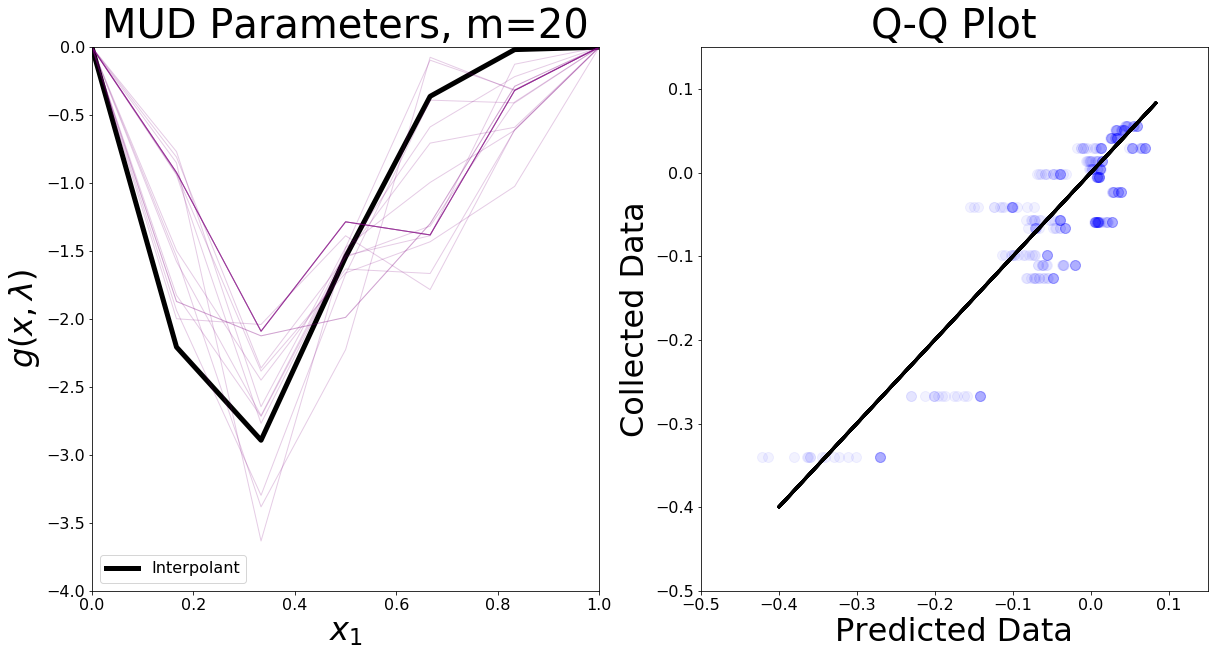
\includegraphics[width=0.95\linewidth]{figures/pde-highd/pde-highd_pair_D-alt-5-1_m20.png}
  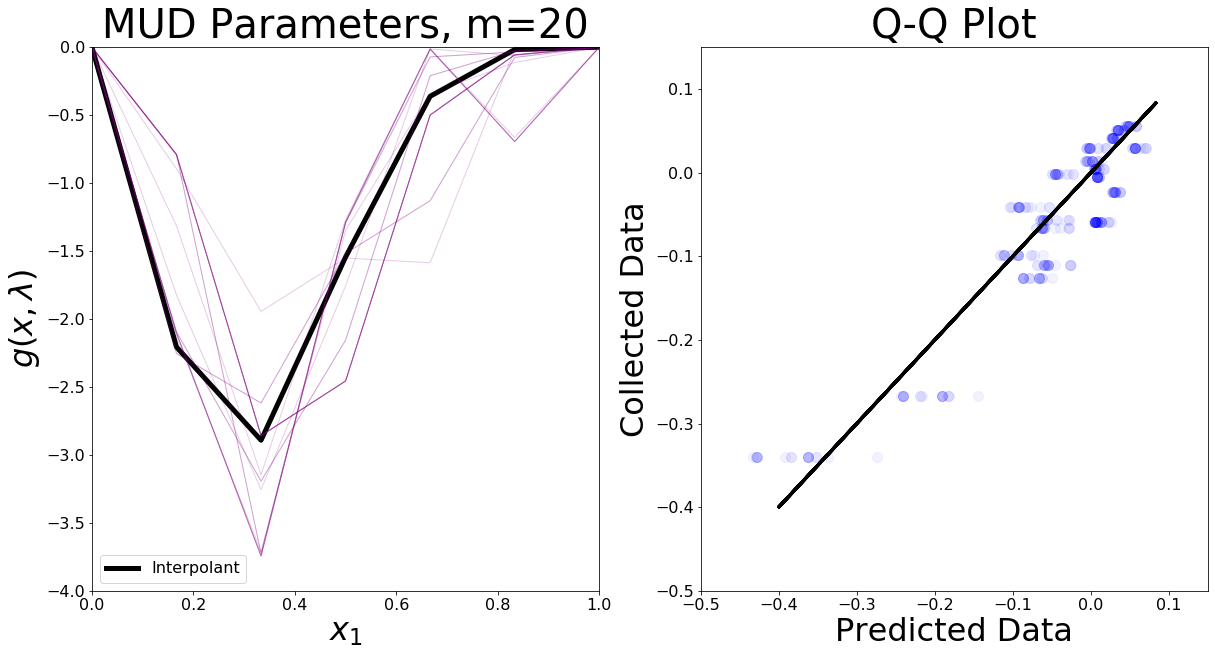
\includegraphics[width=0.95\linewidth]{figures/pde-highd/pde-highd_pair_D-alt-5-5_m20.png}
\caption{Solutions to the SIP using twenty measurements.
(Top): Scalar-valued solutions for alternative approach to the five-dimensional problem.
(Bottom): Vector-valued solutions.
}
\label{fig:pde-highd-5d-alt-mud-20}
\end{figure}

\begin{figure}[htbp]
\centering
  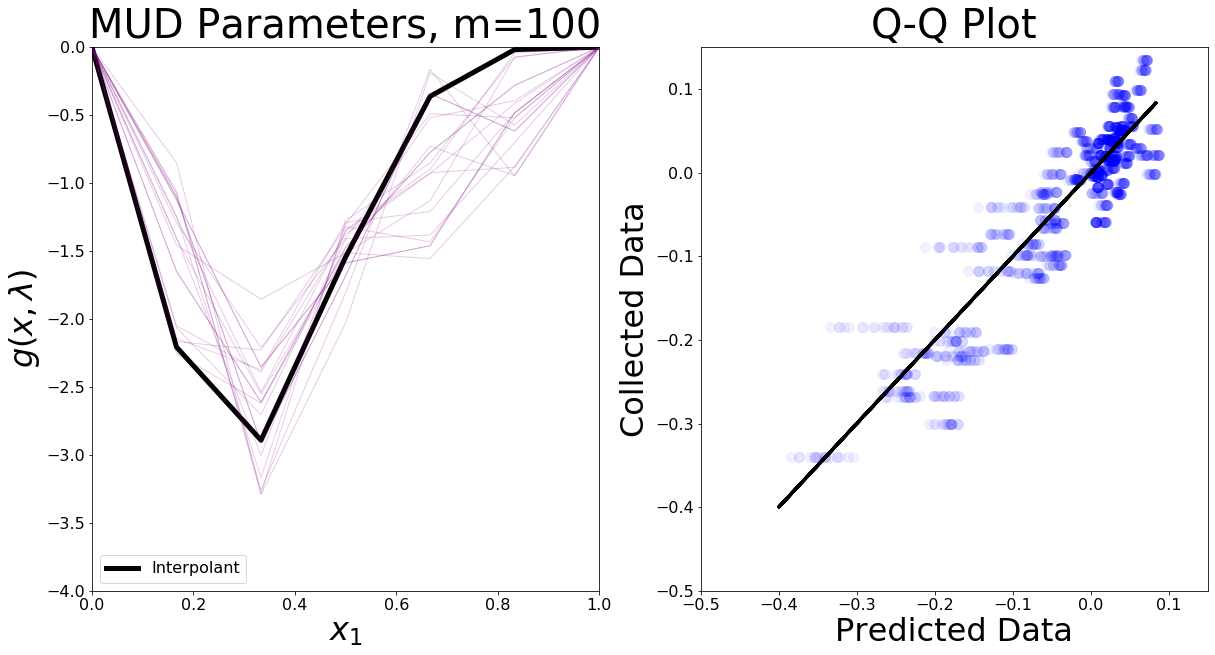
\includegraphics[width=0.95\linewidth]{figures/pde-highd/pde-highd_pair_D-alt-5-1_m100.png}
  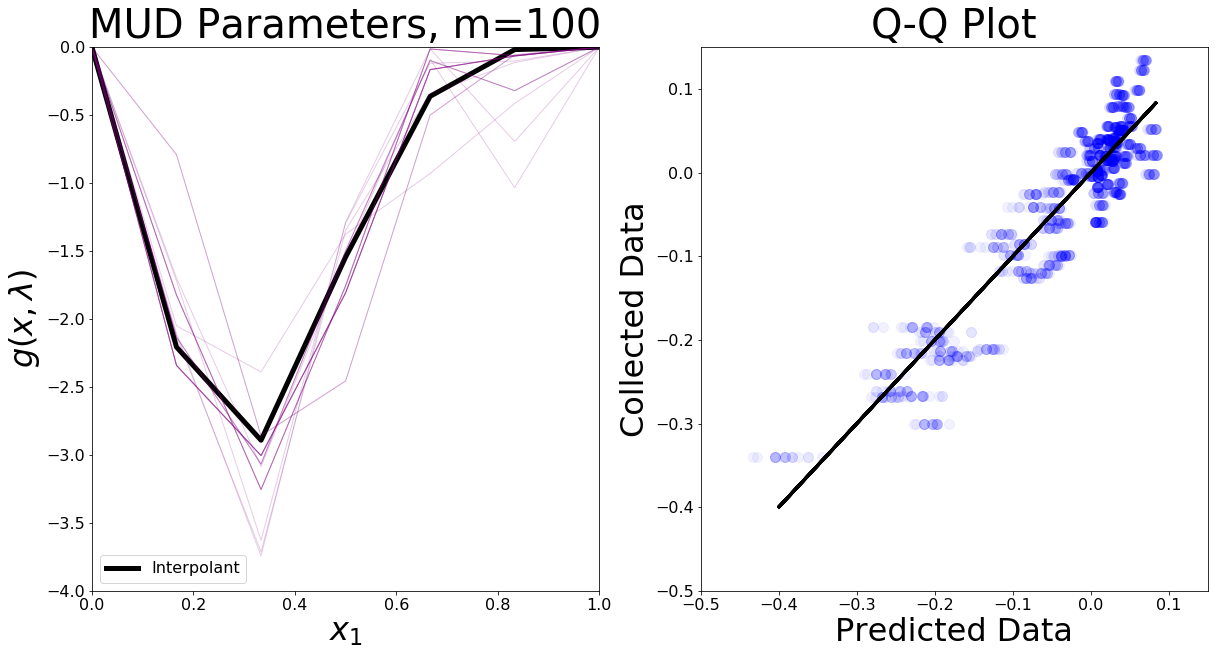
\includegraphics[width=0.95\linewidth]{figures/pde-highd/pde-highd_pair_D-alt-5-5_m100.png}
\caption{Solutions to the SIP using one hundred measurements.
(Top): Scalar-valued solutions for alternative approach to the five-dimensional problem.
(Bottom): Vector-valued solutions.
}
\label{fig:pde-highd-5d-alt-mud}
\end{figure}

Because we began with a better choice of initial density, both QoI maps resolve the residuals similarly (bottom-left of \ref{fig:pde-highd-5d-alt-mud}), and produce qualitatively similar estimates of the response surface. We attribute this to the fact that the vector--valued samples were used to bound the space, but note the direction was informed by the scalar--valued samples.

\subsubsection{Demonstration of Reduction in Uncertainty}

As a final note on this experiment, we contrast the resulting $L^2$-errors to $g$ \footnote{derived from computational approximation with the trapezoidal rule} of these MUD solutions, to the previous two examples in Figure~\ref{fig:pde-highd-5d-hist}, to show a lineage of learning, so to speak.
With each successive problem, our uncertainty is reduced and our MUD solutions lower in variance and increase in accuracy.
Note that they appear to be moving towards a value away from zero, which represents a fixed bias (five equispaced knots can only approximate this $g$ so well).

\begin{figure}[htbp]
\centering
  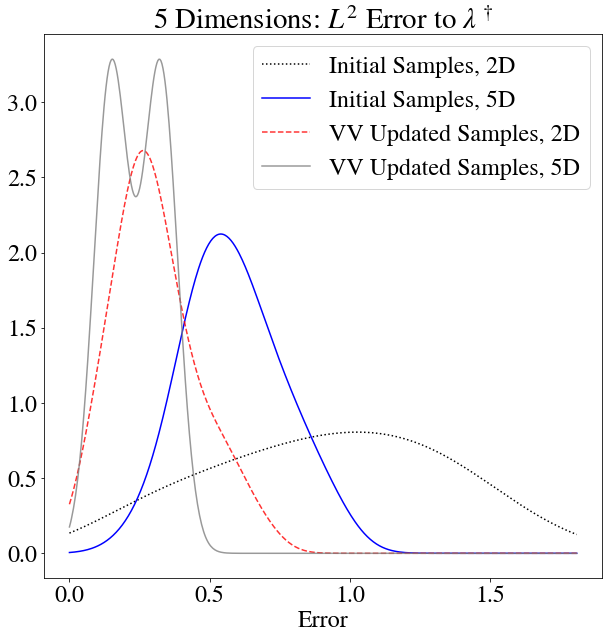
\includegraphics[width=0.675\linewidth]{figures/pde-highd/pde-highd_hist_D5_t5-0E-01}
\caption{
Comparison of the 2D initial errors to the 5D ones, as well as the reduction of uncertainty that solving a SIP problem for each provides.
}
\label{fig:pde-highd-5d-hist}
\end{figure}
